% questions.tex —— 2010 年·普通高等学校招生考试·上海卷·文科 · 题目内容片段（无答案）
% 由 tools/generate_projects.py 依来源总账自 2010/2010_数学真题_上海文_试题.md 生成，勿手改（改源 MD 后重跑）


状态：needs-review；依固定候选 PDF 两页（印刷页 629–630）逐题核验，两幅图已矢量重绘。原页未印分值，不补。

\gkpart{一、填空题}

\begin{question}
\gkti{1}已知集合 $A=\{1,3,m\}$，$B=\{3,4\}$，$A\cup B=\{1,2,3,4\}$，则 $m=$ $\underline{\qquad}$．

\end{question}
\begin{question}
\gkti{2}不等式 $\dfrac{2-x}{x+4}>0$ 的解集是$\underline{\qquad}$．

\end{question}
\begin{question}
\gkti{3}行列式 $\begin{vmatrix}\cos\dfrac\pi6&\sin\dfrac\pi6\\ \sin\dfrac\pi6&\cos\dfrac\pi6\end{vmatrix}$ 的值是$\underline{\qquad}$．

\end{question}
\begin{question}
\gkti{4}若复数 $z=1-2\mathrm i$（$\mathrm i$ 为虚数单位），则 $z\cdot\overline z+z=$ $\underline{\qquad}$．

\end{question}
\begin{question}
\gkti{5}将一个总体分为 $A$、$B$、$C$ 三层，其个体数之比为 $5:3:2$．若用分层抽样方法抽取容量为 $100$ 的样本，则应从 $C$ 层中抽取$\underline{\qquad}$个个体．

\end{question}
\begin{question}
\gkti{6}已知四棱锥 $P-ABCD$ 的底面是边长为 $6$ 的正方形，侧棱 $PA\perp$ 底面 $ABCD$，且 $PA=8$，则该四棱锥的体积是$\underline{\qquad}$．

\end{question}
\begin{question}
\gkti{7}圆 $C:x^2+y^2-2x-4y+4=0$ 的圆心到直线 $l:3x+4y+4=0$ 的距离 $d=$ $\underline{\qquad}$．

\end{question}
\begin{question}
\gkti{8}动点 $P$ 到点 $F(2,0)$ 的距离与它到直线 $x+2=0$ 的距离相等，则点 $P$ 的轨迹方程为$\underline{\qquad}$．

\end{question}
\begin{question}
\gkti{9}函数 $f(x)=\log_3(x+3)$ 的反函数的图象与 $y$ 轴的交点坐标是$\underline{\qquad}$．

\end{question}
\begin{question}
\gkti{10}从一副混合后的扑克牌（$52$ 张）中随机抽取 $2$ 张，则“抽出的 $2$ 张均为红桃”的概率为$\underline{\qquad}$．（结果用最简分数表示）

\Needspace{0.4\textheight}
\end{question}
\begingroup
\renewenvironment{question}{\Needspace{0.5\textheight}}{}
\begin{question}
\gkti{11}$2010$ 年上海世博会园区每天 $9:00$ 开园，$20:00$ 停止入园．在下边的框图中，$S$ 表示上海世博会官方网站在每个整点报道的入园总人数，$a$ 表示整点报道前 $1$ 个小时内入园人数，则空白的执行框内应填入$\underline{\qquad}$．
\nopagebreak[4]
\begin{center}% 2010 年上海卷文科第 11 题：世博入园人数统计程序框图。
% 来源 PDF：普通高考/2010/2010上海文.pdf，SHA-256 5e81bdb27659512a50968275bf502ee666e2ac3f25f9fcaa1b166576fbe9cf62。
% 原页：第 1 页（A3 三栏）第 1 栏下部，书页码 629。
% 重绘依据：T←9、S←0；输出 T,S；判断 T≤19，是则 T←T+1、输入 a、S←S+a 后回到输出，否则结束。
\begin{tikzpicture}[semithick, every node/.style={inner sep=2pt, font=\small}, >=stealth]
  \node[draw,rounded corners] (start) at (0,0) {开始};
  \node[draw,rectangle] (init) at (0,-1.1) {$T\leftarrow9,\ S\leftarrow0$};
  \node[draw,rectangle] (out) at (0,-2.2) {输出 $T,S$};
  \node[draw,diamond,aspect=2] (test) at (0,-3.5) {$T\leqslant19$};
  \node[draw,rectangle] (inc) at (0,-4.7) {$T\leftarrow T+1$};
  \node[draw,rectangle] (inp) at (0,-5.7) {输入 $a$};
  \node[draw,rectangle] (add) at (0,-6.7) {$S\leftarrow S+a$};
  \node[draw,rounded corners] (end) at (3.2,-3.5) {结束};

  \draw[->] (start) -- (init);
  \draw[->] (init) -- (out);
  \draw[->] (out) -- (test);
  \draw[->] (test) -- node[right] {是} (inc);
  \draw[->] (inc) -- (inp);
  \draw[->] (inp) -- (add);
  \draw[->] (add.east) -- (2.0,-6.7) -- (2.0,-2.2) -- (out.east);
  \draw[->] (test) -- node[above] {否} (end);
\end{tikzpicture}
\end{center}
\nopagebreak[4]
\end{question}
\endgroup
\begin{question}
\gkti{12}在 $n$ 行 $n$ 列矩阵

\nopagebreak[4]
\[\begin{pmatrix}
1&2&3&\cdots&n-2&n-1&n\\
2&3&4&\cdots&n-1&n&1\\
3&4&5&\cdots&n&1&2\\
\cdots&\cdots&\cdots&\cdots&\cdots&\cdots&\cdots\\
n&1&2&\cdots&n-3&n-2&n-1
\end{pmatrix}\]

中，记位于第 $i$ 行第 $j$ 列的数为 $a_{ij}$（$i,j=1,2,\cdots,n$）．当 $n=9$ 时，$a_{11}+a_{22}+a_{33}+\cdots+a_{99}=$ $\underline{\qquad}$．

\end{question}
\begin{question}
\gkti{13}在平面直角坐标系中，双曲线 $\Gamma$ 的中心在原点，它的一个焦点坐标为 $(\sqrt5,0)$，$\boldsymbol e_1=(2,1)$，$\boldsymbol e_2=(2,-1)$ 分别是两条渐近线的方向向量．任取双曲线 $\Gamma$ 上的点 $P$，若 $\overrightarrow{OP}=a\boldsymbol e_1+b\boldsymbol e_2$（$a,b\in\mathbf R$），则 $a$、$b$ 满足的一个等式是$\underline{\qquad}$．

\end{question}
\begin{question}
\gkti{14}将直线 $l_1:x+y-1=0$，$l_2:nx+y-n=0$，$l_3:x+ny-n=0$（$n\in\mathbf N^*$，$n\geqslant2$）围成的三角形面积记为 $S_n$，则 $\lim\limits_{n\to\infty}S_n=$ $\underline{\qquad}$．

\end{question}
\gkpart{二、选择题}

\begin{question}
\gkti{15}满足线性约束条件 $\begin{cases}2x+y\leqslant3,\\ x+2y\leqslant3,\\ x\geqslant0,\\ y\geqslant0\end{cases}$ 的目标函数 $z=x+y$ 的最大值是（　）

（A）$1$

（B）$\frac32$

（C）$2$

（D）$3$

\end{question}
\begin{question}
\gkti{16}“$x=2k\pi+\dfrac\pi4$（$k\in\mathbf Z$）”是“$\tan x=1$”成立的（　）

（A）充分不必要条件

（B）必要不充分条件

（C）充要条件

（D）既不充分也不必要条件

\end{question}
\begin{question}
\gkti{17}若 $x_0$ 是方程 $\lg x+x=2$ 的解，则 $x_0$ 属于区间（　）

（A）$(0,1)$

（B）$(1,1.25)$

（C）$(1.25,1.75)$

（D）$(1.75,2)$

\end{question}
\begin{question}
\gkti{18}若 $\triangle ABC$ 的三个内角满足 $\sin A:\sin B:\sin C=5:11:13$，则 $\triangle ABC$（　）

（A）一定是锐角三角形

（B）一定是直角三角形

（C）一定是钝角三角形

（D）可能是锐角三角形，也可能是钝角三角形

\end{question}
\gkpart{三、解答题}

\begingroup
\renewenvironment{question}{\Needspace{0.5\textheight}}{}
\begin{question}
\gkti{19}已知 $0<x<\dfrac\pi2$，化简：

\nopagebreak[4]
\[\lg\left(\cos x\cdot\tan x+1-2\sin^2\frac x2\right)
+\lg\left[\sqrt2\cos\left(x-\frac\pi4\right)\right]
-\lg(1+\sin2x).\]

\Needspace{0.4\textheight}
\end{question}
\endgroup
\begin{question}
\gkti{20}如图所示，为了制作一个圆柱形灯笼，先要制作 $4$ 个全等的矩形骨架，总计耗用 $9.6$ 米铁丝，再用 $S$ 平方米塑料片制成圆柱的侧面和下底面（不安装上底面）．

（1）当圆柱底面半径 $r$ 取何值时，$S$ 取得最大值？并求出该最大值（结果精确到 $0.01$ 平方米）；

（2）若要制作一个如图放置的、底面半径为 $0.3$ 米的灯笼，请作出用于灯笼的三视图（作图时，不需考虑骨架等因素）．
\nopagebreak[4]
\begin{center}% 2010 年上海卷文科第 20 题：圆柱形灯笼（无上底面，四个矩形骨架）。
% 来源 PDF：普通高考/2010/2010上海文.pdf，SHA-256 5e81bdb27659512a50968275bf502ee666e2ac3f25f9fcaa1b166576fbe9cf62。
% 原页：第 2 页（A3 三栏）第 1 栏上部，书页码 630。
% 重绘依据：按底面半径 r、高 h 的圆柱绘制，侧面四条等分竖线表示四个矩形骨架，不画上底面。
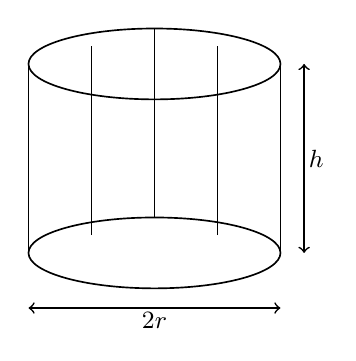
\begin{tikzpicture}[semithick, every node/.style={inner sep=1.4pt, font=\small}]
  % 下底椭圆
  \draw (0,0) ellipse (1.6 and 0.45);
  % 侧边
  \draw (-1.6,0) -- (-1.6,2.4);
  \draw (1.6,0) -- (1.6,2.4);
  % 上口（无上底面，只画椭圆口）
  \draw (0,2.4) ellipse (1.6 and 0.45);
  % 四条骨架竖线
  \draw (-1.6,0) -- (-1.6,2.4);
  \draw (-0.8,0.225) -- (-0.8,2.625);
  \draw (0,0.45) -- (0,2.85);
  \draw (0.8,0.225) -- (0.8,2.625);
  % 标注
  \draw[<->] (-1.6,-0.7) -- (1.6,-0.7);
  \node[below] at (0,-0.7) {$2r$};
  \draw[<->] (1.9,0) -- (1.9,2.4);
  \node[right] at (1.9,1.2) {$h$};
\end{tikzpicture}
\end{center}
\nopagebreak[4]
\end{question}
\begin{question}
\gkti{21}已知数列 $\{a_n\}$ 的前 $n$ 项和为 $S_n$，且 $S_n=n-5a_n-85$，$n\in\mathbf N^*$．

（1）证明：$\{a_n-1\}$ 是等比数列；

（2）求数列 $\{S_n\}$ 的通项公式，并求出使得 $S_{n+1}>S_n$ 成立的最小正整数 $n$．

\end{question}
\begin{question}
\gkti{22}若实数 $x$、$y$、$m$ 满足 $|x-m|<|y-m|$，则称 $x$ 比 $y$ 接近 $m$．

（1）若 $x^2-1$ 比 $3$ 接近 $0$，求 $x$ 的取值范围；

（2）对任意两个不相等的正数 $a$、$b$，证明：$a^2b+ab^2$ 比 $a^3+b^3$ 接近 $2ab\sqrt{ab}$；

（3）已知函数 $f(x)$ 的定义域 $D=\{x\mid x\neq k\pi,\ k\in\mathbf Z,\ x\in\mathbf R\}$．任取 $x\in D$，$f(x)$ 等于 $1+\sin x$ 和 $1-\sin x$ 中接近 $0$ 的那个值．写出函数 $f(x)$ 的解析式，并指出它的奇偶性、最小正周期、最小值和单调性（结论不要求证明）．

\end{question}
\begin{question}
\gkti{23}已知椭圆 $\Gamma$ 的方程为 $\dfrac{x^2}{a^2}+\dfrac{y^2}{b^2}=1$（$a>b>0$），$A(0,b)$、$B(0,-b)$ 和 $Q(a,0)$ 为 $\Gamma$ 的三个顶点．

（1）若点 $M$ 满足 $\overrightarrow{AM}=\dfrac12\left(\overrightarrow{AQ}+\overrightarrow{AB}\right)$，求点 $M$ 的坐标；

（2）设直线 $l_1:y=k_1x+p$ 交椭圆 $\Gamma$ 于 $C$、$D$ 两点，交直线 $l_2:y=k_2x$ 于点 $E$．若 $k_1\cdot k_2=-\dfrac{b^2}{a^2}$，证明：$E$ 为 $CD$ 的中点；

（3）设点 $P$ 在椭圆 $\Gamma$ 内且不在 $x$ 轴上，如何作过 $PQ$ 中点 $F$ 的直线 $l$，使得 $l$ 与椭圆 $\Gamma$ 两个交点 $P_1$、$P_2$ 满足 $\overrightarrow{PP_1}+\overrightarrow{PP_2}=\overrightarrow{PQ}$？令 $a=10$，$b=5$，点 $P$ 的坐标是 $(-8,-1)$．若椭圆 $\Gamma$ 上的点 $P_1$、$P_2$ 满足 $\overrightarrow{PP_1}+\overrightarrow{PP_2}=\overrightarrow{PQ}$，求点 $P_1$、$P_2$ 的坐标．

\end{question}